
% -*- TeX-PDF-mode: t -*-

% -----------------------------------------------
% Template for ISMIR 2010
% (based on earlier ISMIR templates)
% -----------------------------------------------

\documentclass{article}
\usepackage{ismir2010,amsmath,cite}
\usepackage{graphicx}
\usepackage{url}
\usepackage{algorithm,algorithmic}

% added by tbm
\usepackage{subfloat,subfig}
\setlength{\abovecaptionskip}{-3pt}
\setlength{\belowcaptionskip}{6pt} 

\usepackage{booktabs}

\DeclareMathOperator*{\dist}{dist}
\DeclareMathOperator*{\size}{size}

% Title.
% ------
\title{Clustering Beat-Chroma Patterns\\ in a Large Music Database}

% Single address
% To use with only one author or several with the same address
% ---------------
%\oneauthor
% {Names should be omitted for double-blind reviewing}
% {Affiliations should be omitted for double-blind reviewing}

% Two addresses
% --------------
%\twoauthors
%  {First author} {School \\ Department}
%  {Second author} {Company \\ Address}

% Three addresses
% --------------
\threeauthors
  {Thierry Bertin-Mahieux} {Columbia University\\ {\tt tb2332@columbia.edu}}
  {Ron Weiss} {New York University \\ {\tt ronw@nyu.edu}}
  {Dan Ellis} {Columbia University \\ {\tt dpwe@ee.columbia.edu}}
% what order do we use? Thierry, Ron, Dan?  Dan, Thierry, Ron?


% Q: Why are there long spaces after "e.g." or "i.e."?
% A: LaTeX interprets a dot and a blank as the end of a sentence. To
%    prevent this, use "e.g.\ " and "i.e.\ " or "e.g.~" and "i.e.~".
\newcommand{\ie}{i.e.~}
\newcommand{\Ie}{I.e.~}
\newcommand{\eg}{e.g.~}
\newcommand{\Eg}{E.g.~}


\begin{document}
%
\maketitle
%
\begin{abstract}
A musical style or genre implies a set of common conventions
and patterns combined and deployed in different ways to make
individual musical pieces; for instance, most would agree that
contemporary pop music is assembled from a relatively small
palette of harmonic and melodic patterns.  The purpose of this
paper is to use a database of tens of thousands of songs
in combination with a compact representation of melodic-harmonic
content (the beat-synchronous chromagram) and data-mining
tools (clustering) to attempt to explicitly catalog this palette --
at least within the limitations of the beat-chroma representation.
We use online $k$-means clustering to summarize 3.7 million
4-beat bars in a codebook of a few hundred prototypes.
By measuring how accurately such a quantized codebook
can reconstruct the original data, we can quantify the degree
of diversity (distortion as a function of codebook size) and
temporal structure (\ie the advantage gained
by joint quantizing multiple frames) in this music.  The most
popular codewords themselves reveal the common chords
used in the music.  Finally, the quantized representation of
music can be used for music retrieval tasks such as artist
and genre classification, and identifying songs that are
similar in terms of their melodic-harmonic content.
\end{abstract}
%
\section{Introduction}\label{sec:introduction}
The availability of very large collections of music audio present
many interesting research opportunities.  Given millions of examples
from a single, broad class (\eg contemporary commercial pop music),
can we infer anything about the underlying structure and common
features of this class?  This paper describes our work in this direction.

What are the common features of pop music?  There are conventions
of subject matter, instrumentation, form, rhythm, harmony, and melody, among
others.  Our interest here is in the tonal content of the music -- \ie the
harmony and melody.  As a computationally-convenient proxy for a richer
description of the tonal content of audio, we use the popular Chroma
representation, which collapses an acoustic spectrum into a 12-dimensional
description, with one bin for each semitone of the western musical octave.
In addition, we simplify the time axis of our representation to take advantage
of the strong beat present in most pop music, and record just one
chroma vector per beat.  This beat-synchronous chromagram
representation represents a typical music track
in a few thousand values, yet when resynthesized back into audio via
modulation of octave-invariant ``Shepard tones'', the melody and
chord sequences of the original music usually remain recognizable
\cite{Ellis2007a}.  To the extent, then, that beat-chroma
representations preserve tonal content, they
are an interesting domain in which to search for patterns -- rich enough
to generate musically-relevant results, but simplified enough to
abstract away aspects of the original audio such as
instrumentation and other stylistic details.

Specifically, this paper identifies common patterns in beat-synchronous
chromagrams by learning codebooks from a large set of examples.
The individual codewords consist of short beat-chroma patches of
between 1 and 8 beats, optionally aligned to bar boundaries.
%
The additional temporal alignment eliminates redundancy that would be
created by learning multiple codewords to represent the same motive at
multiple beat offsets.
%
The codewords are able to represent the entire dataset
of millions of patterns with minimum error given a small codebook of
a few hundred entries.
%
Our goal is to identify meaningful information
about the musical structure represented in the entire database by
examining individual entries in this codebook.  Since the common
patterns represent a higher-level description of the musical content
than the raw chroma,
we also expect them to be useful in other applications, such as
music classification and retrieving tonally-related items.

Prior work using small patches of chroma features includes
the ``shingles'' of \cite{Casey2007}, which were used to
identify ``remixes'', i.e., music based on some of the same
underlying instrument tracks, and also for matching
performances of Mazurkas \cite{Casey2008}.  That work,
however, was not concerned with extracting the deeper
common patterns underlying different pieces (and did not
use either beat- or bar-synchronous features).  Earlier work in
beat-synchronous analysis includes \cite{Bartsch2001},
which looked for repeated patterns within single songs to
identify the chorus, and \cite{Ellis2007a}, which 
cross-correlated beat-chroma matrices to match cover
versions of pop music tracks.  None of these works
examined or interpreted the content of the chroma
matrices in any detail.  In contrast, here we hope to
develop a codebook whose entries are of interest
in their own right.


\begin{figure}[t]
\begin{center}
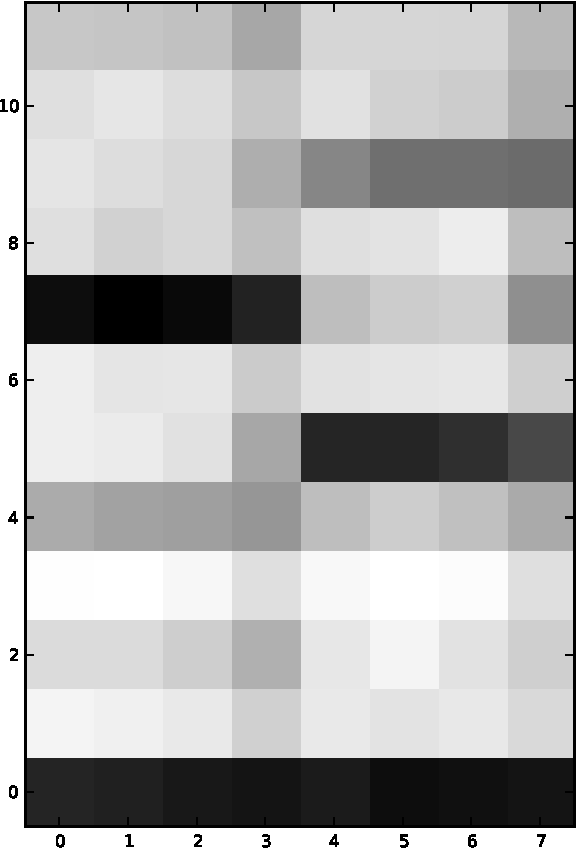
\includegraphics[width=.4\columnwidth]{code}
\end{center}
\caption{\small{A typical codeword from a codebook of size $200$ (code
    7 in Figure \ref{fig:codes1}), corresponding to a
    tonic-subdominant chord progression.  The patch is composed of $2$
    bars and the pattern length was set to $8$ beats.  }}
\label{fig:code}
\end{figure}


\section{Approach}\label{sec:approach}
% In this section we review the creation of the beat-chroma patterns using
% the Echo Nest data.  Then we explain the online vector quantization algorithm
% used to learn a codebook of those patterns.

\subsection{Features}
The feature analysis used throughout this work is based on Echo Nest
analyze API \cite{EchoNest}.  
%
For any song uploaded to their platform this analysis returns a chroma
vector (length $12$) for every music event (called ``segment''), and a
segmentation of the song into beats and bars. Beats may span or 
subdivide segments; bars span multiple beats.
%
Averaging the per-segment chroma over beat times results in a
beat-synchronous chroma feature representation similar to that used in
\cite{Ellis2007a}.  Echo Nest chroma vectors are normalized to have the 
largest value in each column equal to 1.

% \begin{figure}[htb]
% \begin{center}
% 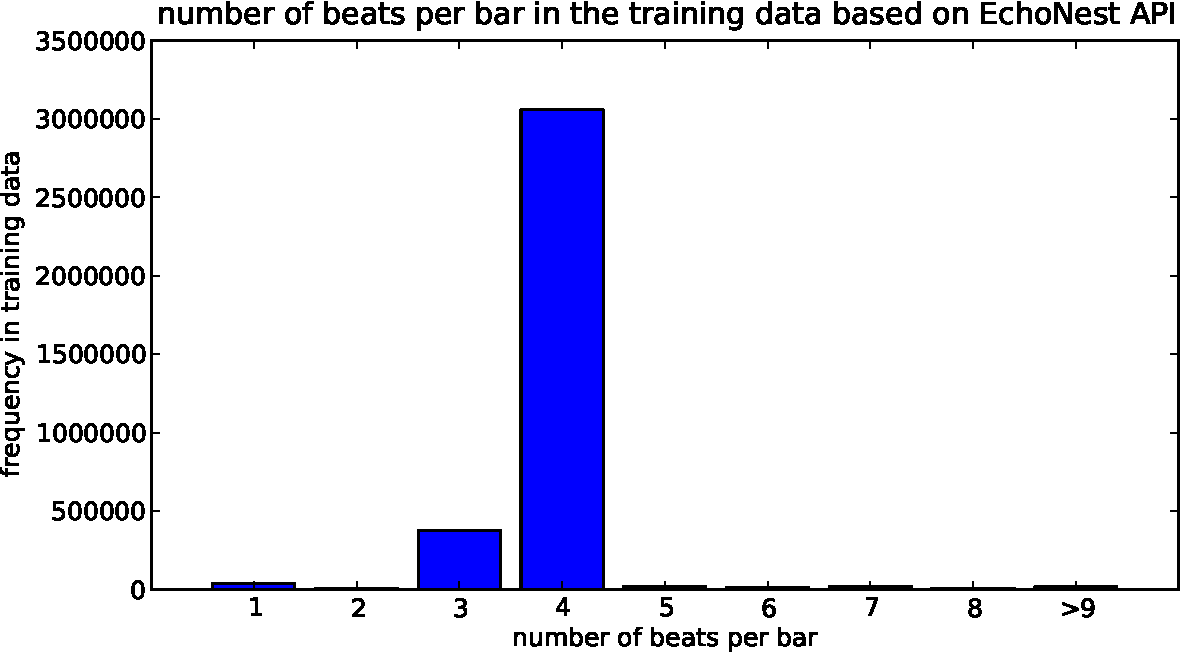
\includegraphics[width=.9\columnwidth]{bar_size_freq}
% \end{center}
% \caption{\small{
% Frequency of the different bar size in the training data.
% }}
% \label{fig:barsize}
% \end{figure}

Note that none of this information (segments, beats, bars)
can be assumed perfectly accurate.
%(\eg in \cite{Barrington2009a} authors obtain a better
%song segmentation than the Echo Nest). 
In practice, we have found them reasonable, 
and given the size of the data set, any rare imperfections or noise
can be diluted to irrelevance by the good examples.  
We also believe that patch sizes based on a number of beats or bars are more
meaningful than an arbitrary time length. This is discussed further in 
Section \ref{ssec:segment}.


%\subsection{Harmonic Patterns}
\subsection{Beat-Chroma Patches} \label{ssec:beatpatch}
% Patterns are defined as a number of beats or bars. In the case of beats,
% we simply cut the set of chromas per beat every $N$ beats. In the case
% of bars, we gather all beats corresponding to the $N$ bars requested.
% The number of chroma vectors we get can vary. We resize the features in the
% time axis to a fixed length. Resizing over clipping can be argued over, 
% but it should
% preserve the main bar characteristics (such as a strong beat at the beginning
% or a note change in the middle).

We use the bar segmentation obtained from the Echo Nest analysis to
break a song into a collection of beat-chroma ``patches'', typically
one or two bars in length.
%
Because the bar length is not guaranteed to be 4 beats, 
depending on the meter of a particular
song, we resample each patch to a fixed length of 4 beats
per bar (except where noted).  However, the majority (82\%) of our training data
consisted of bars that were 4 beats long, so this resampling 
usually had no effect.  Most of the remaining bars (10\%) were 3 beats in
length.
% although the majority of the data contains bars that are 4 beats long
The resulting patches consist of $12 \times 4$ or $12 \times 8$ matrices.

Finally, we normalize the patches with respect to transposition by rotating
the pattern matrix so that the first row contains the most
energy. This can be seen in the example codeword of Figure \ref{fig:code}.
% We considered the same technique for rolling along the other axis and
% be invariant regarding the downbeat. However, it seems less robust to
% noise.
Each patch within a song is normalized independently, so
reconstruction of the original song requires knowledge of the
rotation index for each patch. This rotation removes the key information
of a patch.

The representation resulting from this process is invariant to both
the key and meter of the original song.  This enables the study of
broad harmonic patterns found throughout the data, without regard for
the specific musical context.
%
% In the context of clustering, this enables us to study harmonic
% pattern usage without maintaining clusters for the specific context a
% particular patterns occurs in,
In the context of clustering this avoids problems such as obtaining separate
clusters for every major triad for both duple and triple meters.
% Also, this implies that the pitch envelope is important rather than
% the actual pitches.
%FIXME: Something about why we're not interested in specific chords?
%
%Specific chords do not add much information about a music collection.
%A cover song can be performed in a different key, but the motifs it
%contains remain the same.
%%%% dpwe: I don't agree with this, I'd rather say nothing

\subsection{Clustering}

% We can then stack beat vectors for a number of bars (usually 1 or 2).

We use an online version of the vector quantization algorithm
\cite{Gersho1991} to cluster the beat-chroma patches described in the
previous section.
% This can also be seen as an online K-means.
For each sample from the data, the algorithm finds the closest cluster
in the codebook and updates the cluster centroid (codeword) to be
closer to the sample according to a learning rate $\ell$.
The clusters are updated as each data point is seen, as opposed to
once per iteration in the standard $k$-means algorithm.
The details are explained in Algorithm \ref{algo:vq}.
%
As in standard $k$-means clustering, the codebook is initialized by
choosing $K$ random points from our dataset.
%
Note that this algorithm, although not optimal, scales linearly with
the number of patches seen and can be interrupted at any time
to obtain an updated codebook. %not that this is important...
% The setting of the learning rate might become trickier, but this is
% not fundamentally a problem.

\begin{algorithm}
%\caption{Pseudocode of Vector Quantization}
\begin{algorithmic}
\STATE$\ell$ learning rate
\STATE$\{P_n\}$ set of patches
\STATE$\{C_k\}$ codebook of $K$ codes
%\STATE $m \leftarrow b$
\REQUIRE $0 < \ell \leq 1$
\FOR{$nIters$}
\FOR{$p \in \{P_n\}$}
\STATE$c \leftarrow \min_{c \in C_k} \dist(p,c)$
\STATE$c \leftarrow c + (p - c) * \ell$
\ENDFOR
\ENDFOR
\RETURN $\{C_k\}$
\caption{\small{Pseudocode for the online vector quantization
    algorithm. Note that we can replace the number of iterations by a
    threshold on the distortion over some test set.}
\label{algo:vq}}
\end{algorithmic}
\end{algorithm}



\section{Experiments}\label{sec:experiments}
In this section we present different clustering experiments and introduce
our principal training and test data. Some detailed settings
of our algorithm are also provided. As for any clustering algorithm, we
measure the influence of the number of codewords and the training set size.


\subsection{Data}
%\subsection{Training data: Cowbell Dataset}
\label{sec:traindata}
%\subsection{Test data: USPOP}
\label{sec:testdata}
Our training data consists of $43,300$ tracks that were uploaded to
morecowbell.dj,\footnote{http://www.morecowbell.dj/} an online service
based on the Echo Nest analyze API which remixes uploaded music by
adding cowbell and other sound effects synchronized in time with the
music.  The $43.3$K songs contain $3.7$ million non-silent
bars which we clustered using the approach described in the previous
section.

For testing, we made use of low quality (32kbps, 8 kHz bandwidth mono MP3) versions of the songs
from the {\it uspop2002} data set \cite{uspop2002}.  This well-known data set 
contains pop songs from a range of artists and styles.
% \footnote{We also tried to use Tzanetakis dataset,
% %\cite{Tzanetakis2002a},
% but the $30$ seconds segments seemed hard to analyze by the Echo Nest API, 
% most did not contain any bar.}.
{\it uspop2002} serves as test set to measure how well a codebook learned on
the Cowbell data set can represent new songs.  We obtained Echo Nest features
for the $8651$ songs contained in the dataset.


\subsection{Settings}\label{ssec:setting}
We take one or two bars and resample the patches to 4 or 8 columns 
respectively.  We learn a codebook of size $K$ over the Cowbell
dataset using the online VQ algorithm (Algorithm \ref{algo:vq}). We use a
learning rate of $\ell=0.01$ for $200$ iterations over the whole
dataset.
%
We then use the resulting codebook to encode the test set.
Each pattern is encoded with only one code. We can measure the average
distance between a pattern and its encoding. We can also measure the use
of the different codes, 
%\ie the size of the cluster around a code.
i.e., the proportion of patterns that quantize to each code.

We use the average squared Euclidean distance as the distortion
measure between chroma patches.  Given a pattern $p_1$
composed of elements $p_1(i,j)$, and a similar pattern $p_2$, the
distance between them is:
\begin{eqnarray}
  \dist(p_1,p_2) = \sum_{i,j} \frac{(p_1(i,j) - p_2(i,j))^2}{\size(p_1)}
  \label{eq:dist}
\end{eqnarray}
We assume $p_1$ and $p_2$ have the same size.  This is enforced by the
resampling procedure described in Section \ref{sec:approach}.


\begin{figure}[t]
\begin{center}
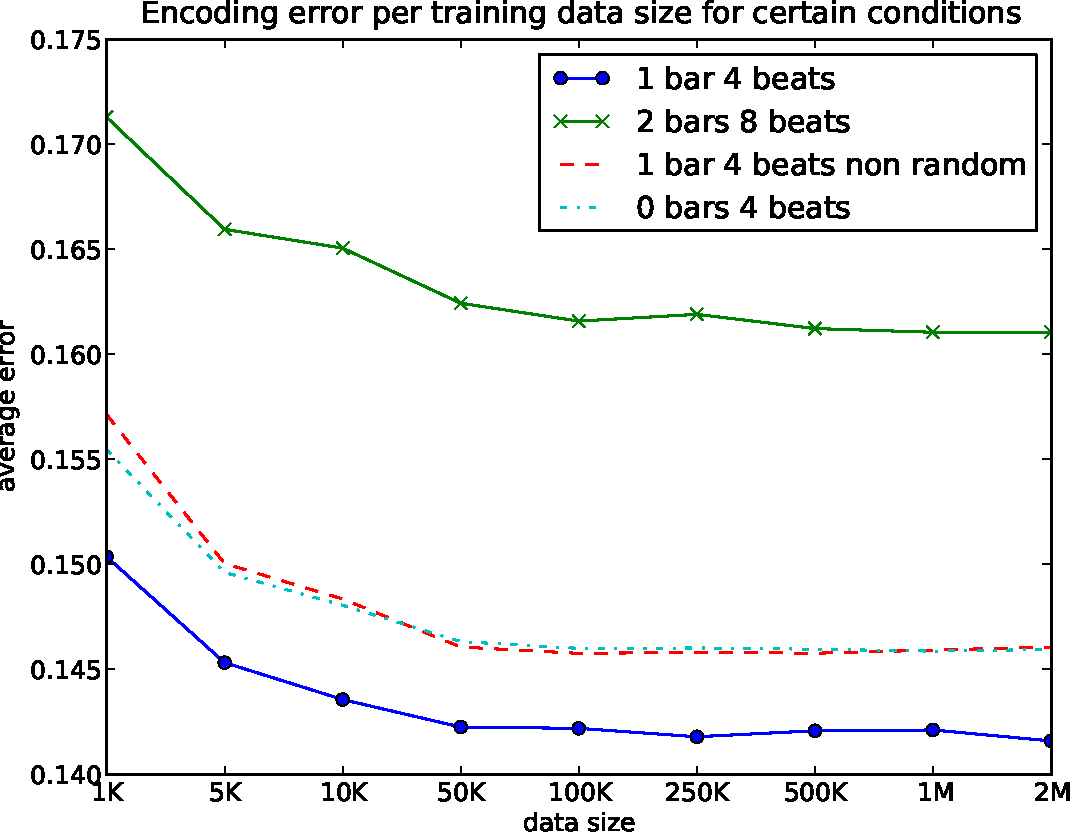
\includegraphics[width=.8\columnwidth]{data_sizes}
\end{center}
\caption{\small{Distortion for a codebook of size $100$ encoding one bar
at a time with by $4$ columns.
Therefore, each codeword has $12 \times 4 = 48$ elements.
Distortion is measured on the test set.  Training data sizes range
from $0$ (just initialization) to $500,000$. Patterns were selected at
random from the dataset of approximately $3.7$ million patterns.
}}
\label{fig:data_sizes}
\end{figure}


\subsection{Codebook properties}
This section presents some basic results of the clustering.
While unsurprising, these results may be useful for comparison 
when reproducing this work.
\begin{itemize}
\item Encoding performance improves with increasing training data (Figure
\ref{fig:data_sizes}). Distortion improvements plateau by around $1000$ samples 
per codeword ($100,000$ samples for the $100$-entry codebook of the figure).
\item Encoding performance improves with increasing codebook size
(Table \ref{tab:cbsize}).  Computation costs scales with codebook size, 
which limited the largest codebooks used in this work, but larger codebooks 
(and more efficient algorithms to enable them) are clearly a promising future 
direction.
\item Larger patterns are more difficult to encode, thus requiring
larger codebooks. See Figure \ref{fig:perbeat}. The increase is steepest
below $4$ beats (1 bar), although there is no dramatic change at 
this threshold.
\end{itemize}


\begin{table}
\begin{center}
\begin{tabular}{llc}
\toprule
Codebook size & Distortion \\
\midrule
1 & $0.066081$ \\
10 & $0.045579$ \\
50 & $0.038302$ \\
100 & $0.035904$ \\
500 & $0.030841$ \\
\bottomrule
\end{tabular}
\end{center}
\caption{\small{Distortion as a function of codebook size for a fixed training set 
of $50,000$ samples.  Codebook consists of $1$ bar ($4$ beat) patterns.
  }}
\label{tab:cbsize}
\end{table}


\begin{figure}[b]
\begin{center}
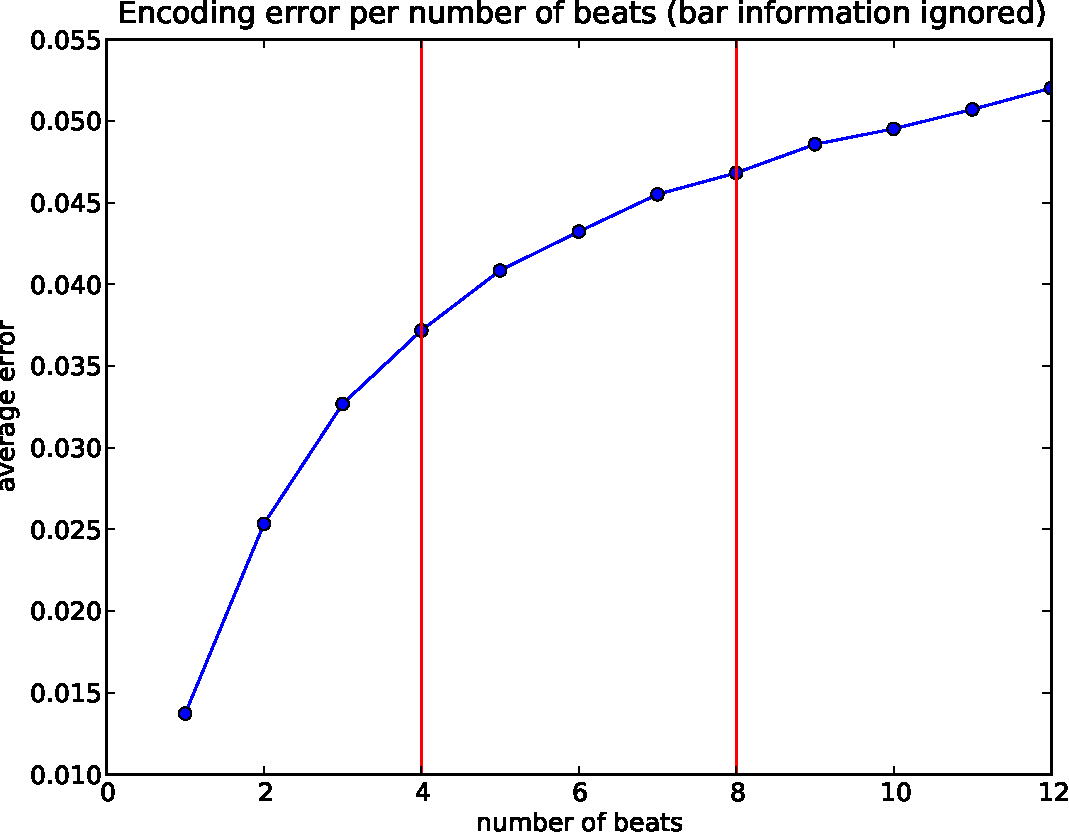
\includegraphics[width=.8\columnwidth]{encoding_per_beat}
\end{center}
\caption{\small{Encoding patterns of different sizes with a fixed size
codebook of 100 patterns. The size of the pattern is defined by the number of beats. 
Downbeat (bar alignment) information was not used for this experiment. % why not?
}}
\label{fig:perbeat}
\end{figure}


\section{Visualization} \label{sec:visu}
% The goal here is to give an intuition to the reader of what kind of
% typical patterns do we get. We also want to have a feel for what the
% clusters look like, how many boring sustained notes are encoded in the
% codebook, can the codebook describes the complexity of the music space, etc.


\subsection{Codebook}\label{sec:codebook}

We trained a codebook $200$ entries of patterns sized $12\times8$, covering
$2$ bars at a time.  The results shown are on the {\it artist20} test set described in 
Section \ref{ssec:artist}.


\begin{figure}[t]
\begin{center}
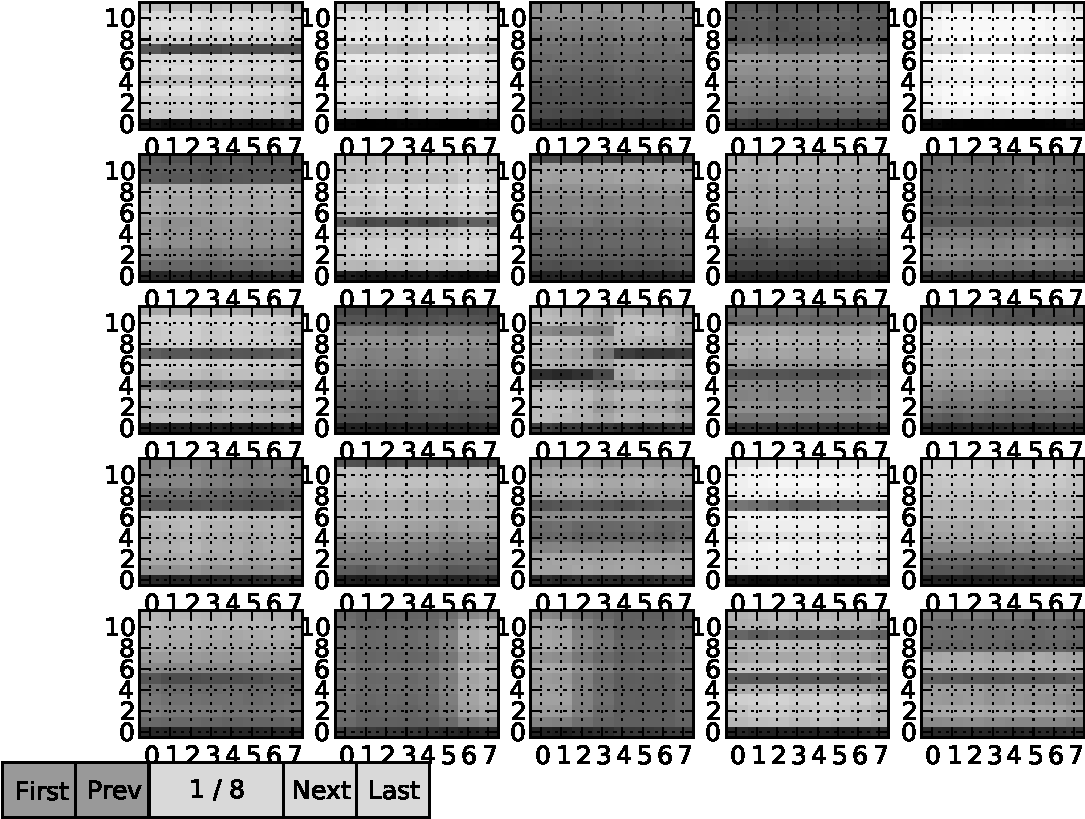
\includegraphics[width=\columnwidth]{codes1}
\end{center}
\caption{\small{
The 25 codes that are 
most commonly used for the {\it artist20} test set. 
Codes are from the $200$-entry codebook trained on $2$ bar, $12 \times 8$
patches.  The proportion of patches accounted for by each pattern is shown 
in parentheses.
%There are $71832$ patterns in total in the dataset.
}}
\label{fig:codes1}
\end{figure}

\begin{figure}[bt]
\begin{center}
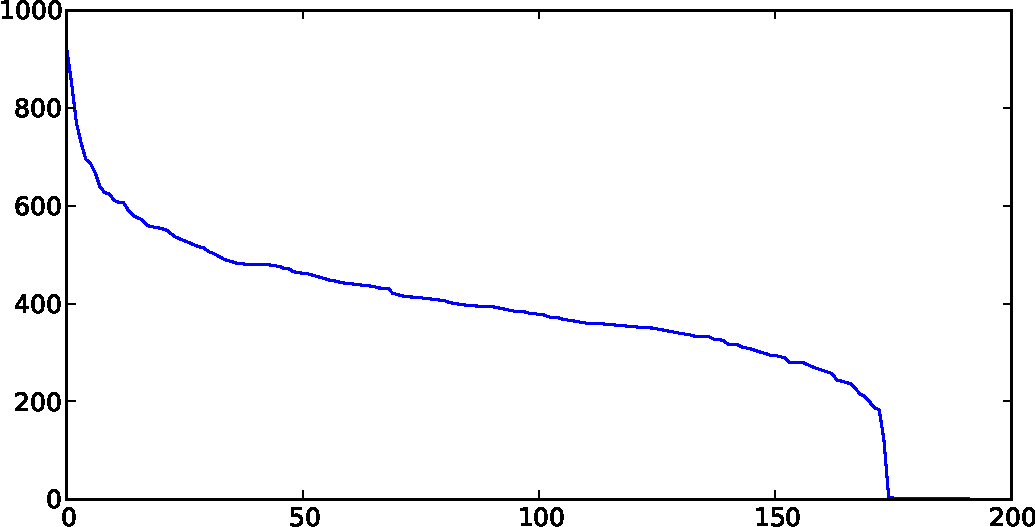
\includegraphics[width=.99\columnwidth]{freqs}
\end{center}
\caption{\small{Usage proportions for all 200 codewords 
on the {\it artist20} test set (which comprises $71,832$
patterns).  Also shown are the usage proportions for the training set (``cowbell''), 
which are similar.
Note that even though all codewords are initialized from samples, some
are used only once in the training set, or not at all for test set.
This explains why the curves drop to $0$.
}}
\label{fig:freqs}
\end{figure}

The 25 most frequently used codewords in the test set are shown in
Figure \ref{fig:codes1}.  
The frequency of use of these codewords is shown in Figure \ref{fig:freqs}.
The codewords primarily consist of sustained
notes and simple chords.  Since they are designed to be key-invariant,
specific notes do not appear.  Instead the first 7 codewords
correspond to a single note sustained across two bars (codeword 0),
perfect fifth (codewords 1 and 2) and fourth intervals (codewords 3
and 6, noting that the fourth occurs when the per-pattern transposition 
detects the fifth rather than the root as the strongest chroma bin, and vice-versa), and a
major triads transposed to the root and fifth (codewords 5 and 4, respectively).  Many of the remaining
codewords correspond to common transitions from one chord to another,
\eg a V-I transition in codes 7 and 9
(e.g., Gmaj
$\rightarrow$ Cmaj, or G5 $\rightarrow$ C5 as a guitar power chord)
% assuming that chroma 0 is C) 
and the reverse I-V transition in code 21 (e.g., Cmaj
$\rightarrow$ Gmaj).
%FIXME: Does this transition have a better name like ``relative x''?
% C5 -> F5 in 'guitar chords', basically a power chord

\begin{figure}[t]
\begin{center}
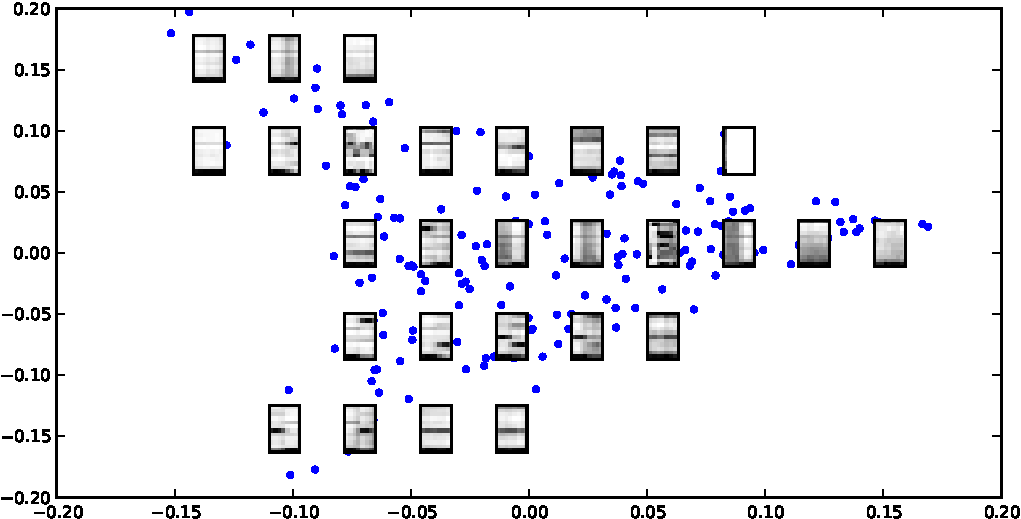
\includegraphics[width=.9\columnwidth]{codes_lle}
\end{center}
\caption{\small{
LLE visualization of the codebook.
%LLE tries to keep near neighbors (here according to euclidean distance)
%in the same $2$D neighborhood. 
Shown patterns are randomly selected
from each neighborhood.
}}
\label{fig:lle}
\end{figure}

In an effort to visualize the span of the entire codebook, we used 
Locally linear embedding (LLE) \cite{Roweis2000}\footnote{implementation:
  \url{http://www.astro.washington.edu/users/vanderplas/coding/LLE/}}
to arrange the codewords on a 2D plane while keeping similar 
patterns as neighbors.  Figure \ref{fig:lle} shows the resulting 
distribution along with a sampling of patterns; notice 
% ron's text instead of Dan
sustained
chords on the top left, chord changes on the bottom left, and more
complex sustained chords and ``wideband'' noisy patterns grouping to
the right of the figure.

%trends such as the 
%more ``wideband'' patterns to the right.

%Another interesting visualization uses LLE\footnote{implementation:
%  \url{http://www.astro.washington.edu/users/vanderplas/coding/LLE/}}
%algorithm \cite{Roweis2000} to display codewords arranged in
%coherent groups. See Figure \ref{fig:lle}. For instance, we see
%``wideband'' patterns grouping to the right.

\begin{figure}[t]
\begin{center}
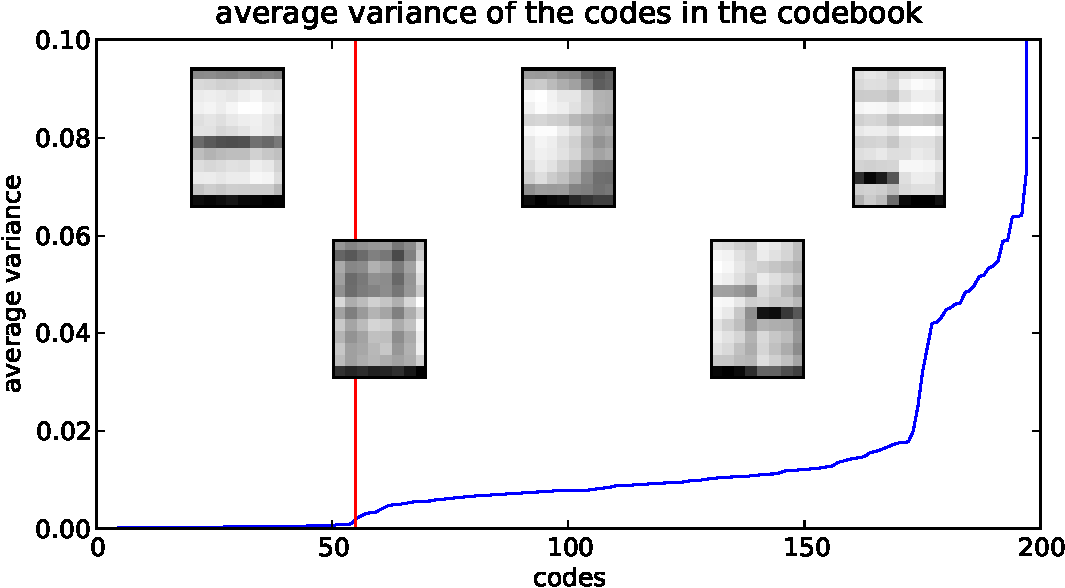
\includegraphics[width=.9\columnwidth]{code_variance}
\end{center}
\caption{\small{Average variance of codewords along the time dimension. The vertical
axis cuts at the $53$rd pattern, roughly the number of 
codewords consisting entirely of sustained chords.  Representative patterns are shown 
in each range.
}}
\label{fig:code_var}
\end{figure}

Noting that many of the codewords reflect sustained patterns with 
little temporal variation, Figure \ref{fig:code_var} plots the average 
variance along time of all 200 patterns.  
Some 26\% of the codewords have very low variance, corresponding 
to stationary patterns similar to the top row of Figure
\ref{fig:codes1}. 
%For $2$ bars codewords, it seems that patterns
%containing more complex temporal activity account for only $33$\% of
%the data.
%%%% dpwe: I can't tell what this means, so drop it.

\begin{figure}[htb]
\begin{center}
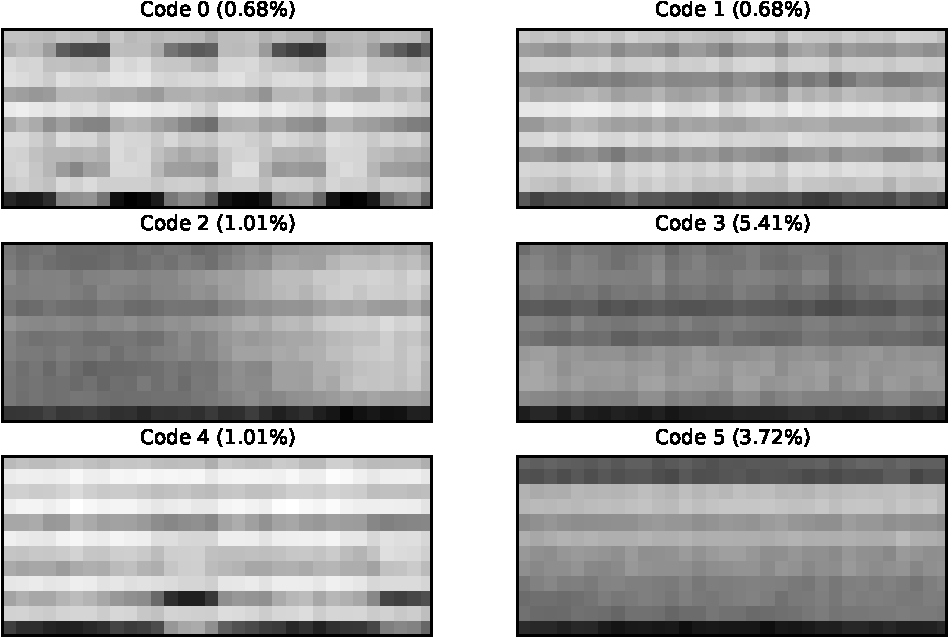
\includegraphics[width=.8\columnwidth]{codes_8bars}
\end{center}
\caption{\small{Sample of longer codewords spanning $8$
    bars. Codewords were randomly selected from a 100-entry 
    codebook. Percentages of use are shown in parentheses.  Most patterns
    consist of sustained notes or chords, but code 0 shows one-bar 
    alternations between two chords, and code 4 contains two cycles of a
    1$\rightarrow$1$\rightarrow$1$\rightarrow$2 progression.}}
\label{fig:codes8bars}
\end{figure}

We made some preliminary experiments with codebooks based on 
longer patches.  Figure \ref{fig:codes8bars} presents a codewords 
from an 8 bar (32 beat) codebook.  We show a random selection 
since all the most-common codewords were less interesting, sustained 
patterns.

%Showing codewords of $2$ bars is practical and consistent with our experiments
%in Section \ref{sec:exps2}. However, longer codewords can also reveal
%interesting structure. A random sample of such codewords is presented
%in Figure \ref{fig:codes8bars}. Most used codewords would be less interesting,
%as they all are sustained patterns.

\begin{figure}[t]
\begin{center}
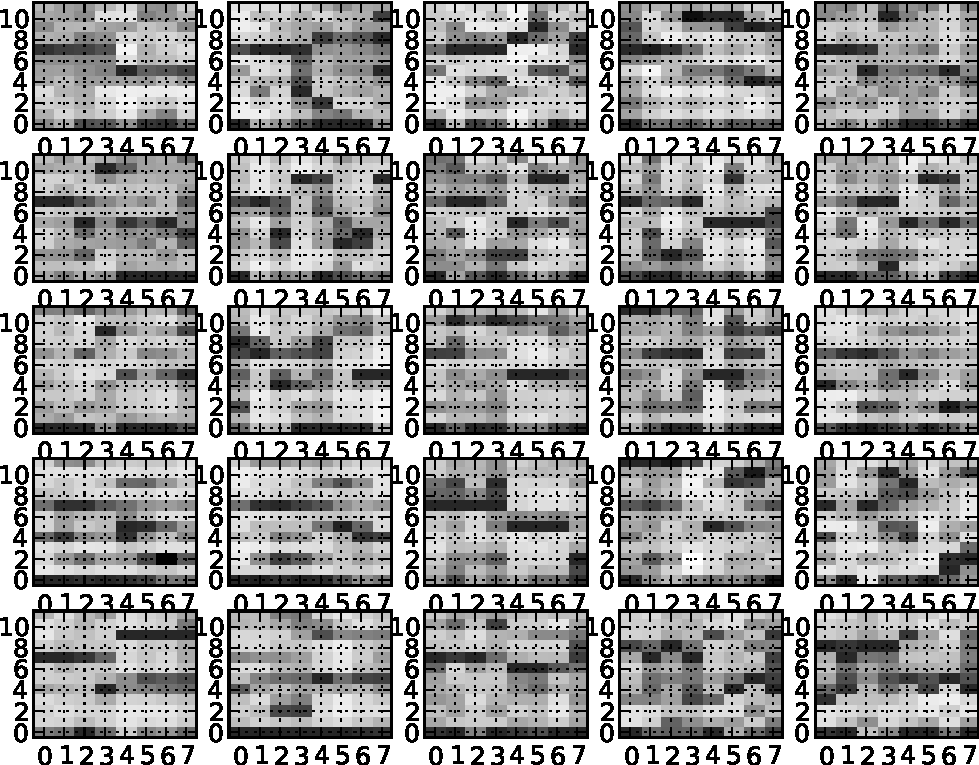
\includegraphics[width=.95\columnwidth]{close_patterns1}
\end{center}
\caption{\small{Cluster around centroid presented in
Figure \ref{fig:code}. Taken from the {\it artist20} dataset, the cluster
size is actually $639$. Shown samples were randomly selected.
This gives an intuition of the variance
in a given cluster.
}}
\label{fig:cluster}
\end{figure}

\subsection{Within-cluster behavior}
In addition to inspecting the codewords, it is important to understand 
the nature of the cluster of patterns represented by each codeword, i.e., 
how well the centroid describes them, and the kind of detail that has 
been left out of the codebook.  Figure \ref{fig:cluster} shows a random 
selection of the $639$ patterns from the {\it artist20} test set that 
were quantized to codeword 7 from Figure \ref{fig:codes1}, the V-I cadence. 
Figure \ref{fig:cluster_diff} illustrates the difference between the actual 
patterns and the quantized codeword for the first three patterns; although 
there are substantial differences, they are largely unstructured, indicating 
that the codebook has captured the important underlying trend.

%Visualizing a codebook is half of the story, we also want to understand
%clusters, \ie the patterns from actual song that
%surround a given centroid (codeword). Unsurprisingly, real patterns are
%noisier than codes. However, centroids seem to capture important aspects
%of the patterns. We could compare the centroids with the result of
%a lowpass filtering. In Figure \ref{fig:cluster} we show elements of the same
%cluster, and in Figure \ref{fig:cluster_diff}, we emphasize the difference
%with the centroid. We hope for the difference to look uniformly random,
%the result seems to fit that assumption.

%FIXME: we want the differences to be close to uniformly random, right
%(hence centroid)?
%And that's kind of what they look like.  Does Fig
%\ref{fig:cluster_diff} really add much?


\begin{figure}[t]
\begin{center}
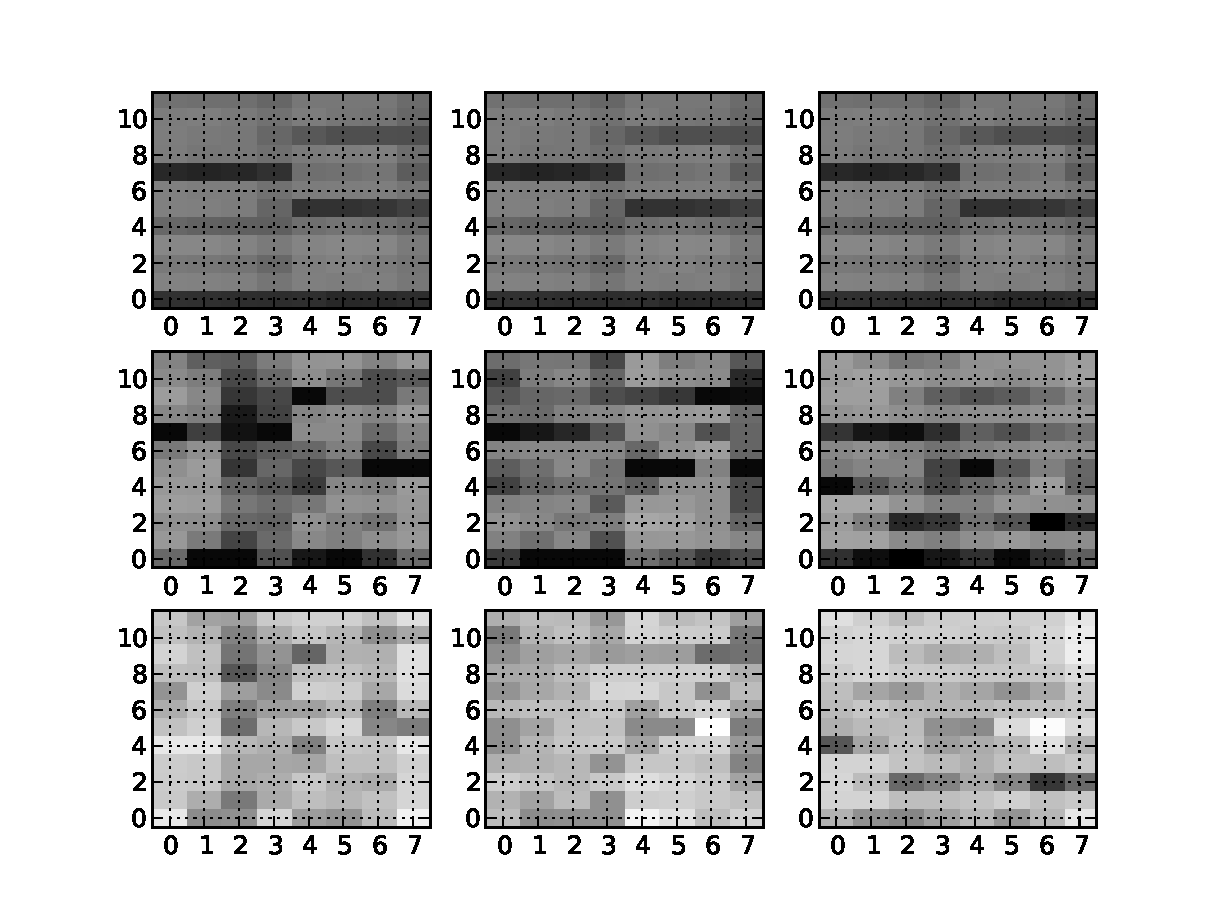
\includegraphics[width=.95\columnwidth]{close_patterns_diff}
\end{center}
\caption{\small{First three patterns of figure \ref{fig:cluster}
($2$nd line) presented with the centroid from Figure \ref{fig:code}
($1$st line) and the absolute difference between both ($3$rd line).
}}
\label{fig:cluster_diff}
\end{figure}


\subsection{Example song encoding}

Figure \ref{fig:encodesong} gives an example of encoding a song
using the codebook, showing both the full, original data, and the 
reconstruction using only the quantized codewords (at the correct transpositions).  
The quantized representation retains
the essential harmonic structure of the original features, but has smoothed
away much of the detail below the level of the 2 bar codewords.
%
%This is consistent with the codebook described in Section
%\ref{sec:codebook} which primarily consists of sustained chords across
%4 or 8 beats.

\begin{figure}[htb]
\begin{center}
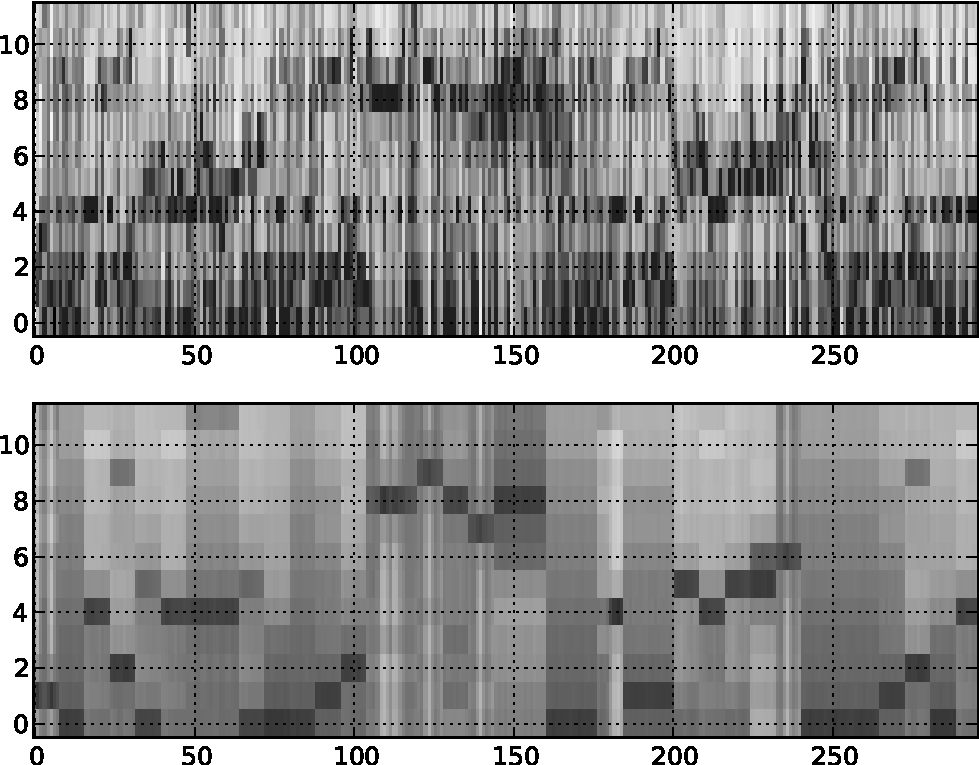
\includegraphics[width=.9\columnwidth]{song_encoded}
\end{center}
\caption{\small{Good Day Sunshine by \textit{The Beatles}.
Original song and encoding with a $200$ entry codebook of 
$2$ bar patterns.
}}
\label{fig:encodesong}
\end{figure}


\section{Applications}\label{sec:exps2}
We present two applications of the beat-chroma codebooks
to illustrate how the ``natural'' structure identified via 
unsupervised clustering can provide useful 
features for subsequent supervised tasks.  We will discuss how 
the codewords can be used in song segmentation, and for artist
recognition.  
%The representation created from large collections
%captures meaningful information without being forced to do so.
%
% Although our algorithm was not devised for any of these
% tasks, but some information contained in the centroids can be
% naturally used.

\subsection{Song Segmentation} \label{ssec:segment}

Since the clustering described in Section \ref{sec:approach} is based
on the segmentation of the signal in to bars, 
the codewords should contain information related to bar
alignment, such as the presence of a strong beat on the first beat.
%
In this section we investigate using the codebook to identify the
bar segmentation of new songs.  
% using the information contained in the cluster centroids.  
We train a codebook of size $100$ on bars resampled to $4$ beats. Then,
we take the longest sequence of bars of $4$ beats for each song
in the test set (to avoid the alignment skew that results from spanning 
irregularly-sized bars).  
%As we mentioned before, $4$ beats is the most common bar size using the
%Echo Nest segmentation. 
We then encode each of these sequences using an offset
of $0$, $1$, $2$ or $3$ beats, and record for each song 
the offset giving the lowest distortion.  
%The best offset for a test sequence
%(the one with the lowest distortion)
%should correspond to the bar alignment in the original
%feature matrix.  
%The correct answer is an offset of $0$.
%
The results in Table \ref{tab:offset}
show that the ``true'' offset of $0$ beats is chosen in $62\%$ of cases (where a random 
guess would yield $25\%$).  Thus, the codebook is useful for identifying bar (downbeat) 
alignments.  A more flexible implementation of this idea would use dynamic 
programming to align bar-length patterns to the entire piece, including the 
possibility of 3- or 5-beat bars (as are sometimes needed to accommodate 
beat tracking errors) with an appropriate associated penalty.  

%FIXME: Actually I'm (ronw) not sure how this was done.  Every 4 beat
%segment was treated separately?  Its not looking for a per-song alignment?
%TBM: yes, I simply summed the divergence from all patterns for a given
% divergence, the lowest sum is the winner. So it's a per-song alignment.

%The result presented here suggest a dynamic programming setting where
%we could find the optimal bar segmentation according to our codebook. 
%We could try
%all possible bar length (in terms of beats) and not restrict ourselves
%to $4$ beats bars and offsets between $0$ and $3$. This is part of
%our future work.

\begin{table}
\begin{center}
\begin{tabular}{cc}
\toprule
Offset & \% of times chosen \\
\midrule
0 & $\mathbf{62.6}$\\
1 & $16.5$\\
2 & $\text{ }9.4$\\
3 & $11.5$\\
\bottomrule
\end{tabular}
\end{center}
\caption{\small{
Song segmentation experiment:
offsets relative to ground-truth 4-beat bar boundaries 
that gave minimum distortion encodings from the bar-aligned codebook.
%The real one is $0$.
%Random guess gives an accuracy of $25$\%.
}}
\label{tab:offset}
\end{table}

\subsection{Artist Recognition} \label{ssec:artist}

We apply our codebook to a simple artist recognition task.
We use the {\it artist20} data set, composed of $1402$ songs from $20$ artists, 
mostly rock and pop of different subgenres.  
Previously published results using GMMs on MFCC features achieve an 
accuracy of $59\%$, whereas using only chroma as a representation yields an
accuracy of $33\%$  \cite{Ellis2007}. 

Although beat-chroma quantization naturally discards information 
that could be useful in artist classification, it is interesting to 
investigate whether some artist use certain patterns more often than others.

The dataset is encoded as histograms of the codewords 
used for each song, with frequency values normalized by the number
of patterns in the song. We test each song in a leave-one-out setting, 
and represent each of the $20$ artists by the average of their (remaining) 
song-histograms.  The test song is matched to an artist based on 
minimum Euclidean distance to these per-artist averages.
This gives an accuracy of $23.4\%$, where the random baseline 
is around $5\%$. 
The confusion matrix can be seen in Figure \ref{fig:conf_mat}, showing 
that certain artists are recognized at an accuracy far above the average.

\begin{figure}[t]
%\begin{center}
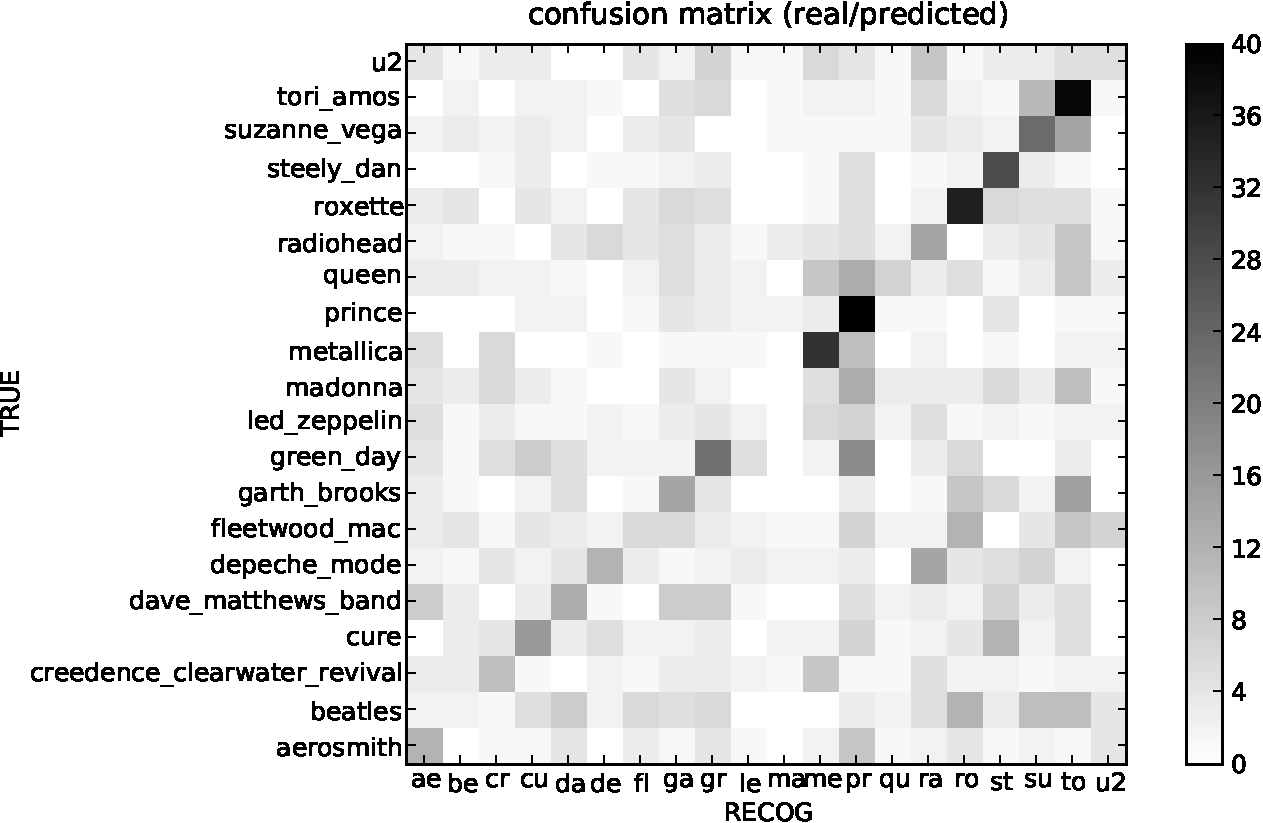
\includegraphics[width=.9\columnwidth]{conf_mat_per_artist}
%\end{center}
\caption{\small{Confusion matrix for the artist recognition task.}}
\label{fig:conf_mat}
\end{figure}

%Looking at the most typical patterns per artist can be insightful.
It is interesting to inspect the most ``discriminative'' patterns for 
individual artists.  
To find these patterns, we compare a pattern's use by one artist and divide
by its use across all artists. Figure \ref{fig:typicalpat} 
shows the dominant patterns for Metallica, and for Tori Amos and
Suzanne Vega (who shared a `favorite' pattern). 
These three artists were easily identified.
Artists like Metallica are characterized by ``wideband'' patterns, 
with energy spread across multiple adjacent chroma bins, 
indicative of noise-like transients in the audio.
%FIXME: ron, what di you mean: (not by cleaned up by EN's feature analysis)

% ignoring the two following figures
\iffalse
\begin{figure}[htb]
\begin{center}
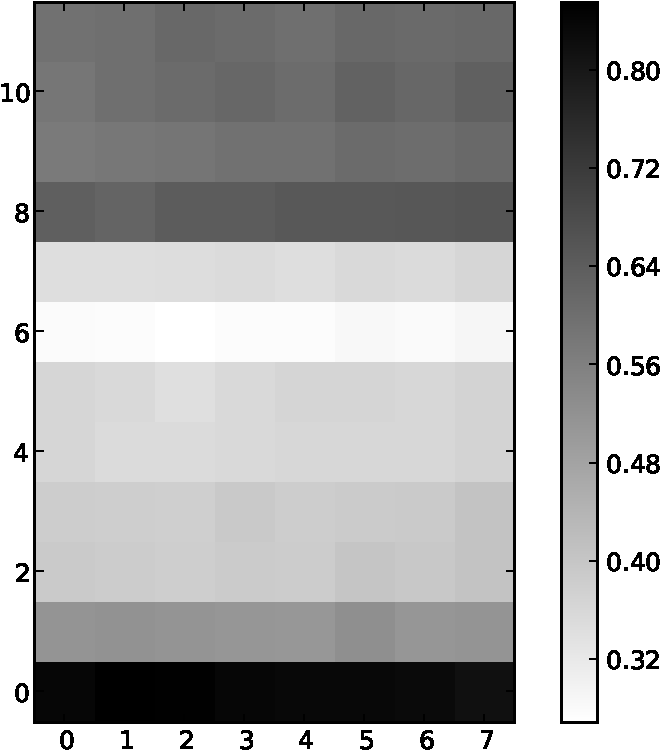
\includegraphics[width=.4\columnwidth]{metallica_pattern}
\end{center}
\caption{\small{Most typical pattern for Metallica.
COULD BE MIXED WITH TORI AMOS FIGURE.
}}
\label{fig:metallica}
\end{figure}

\begin{figure}[htb]
\begin{center}
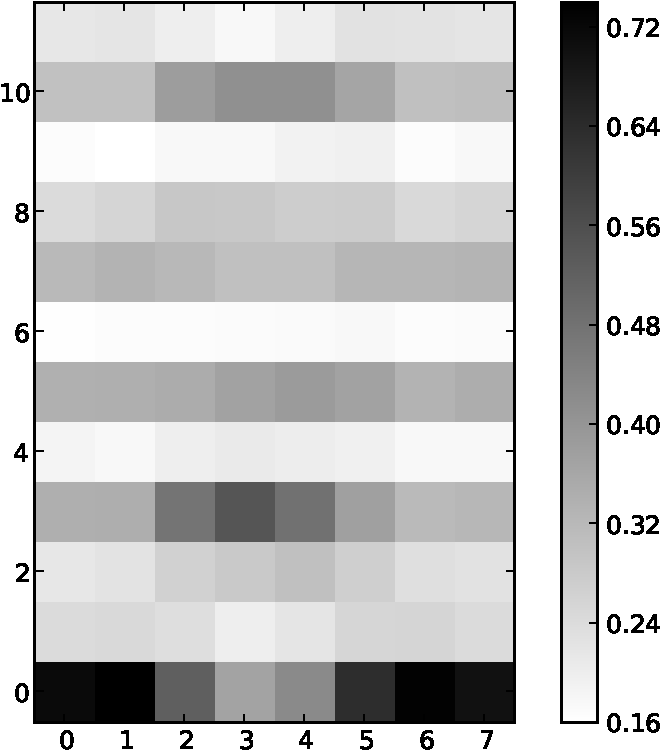
\includegraphics[width=.4\columnwidth]{toriamos_suzannevega_pattern}
\end{center}
\caption{\small{Most typical pattern for Tori Amos and Suzanne Vega.
    Can we show the top 2 or 4 for each to get a better idea?}}
\label{fig:amosvega}
\end{figure}
\fi


\begin{figure}[h]
  \centering
  \subfloat[][\small{Metallica}]{\label{fig:metallica2}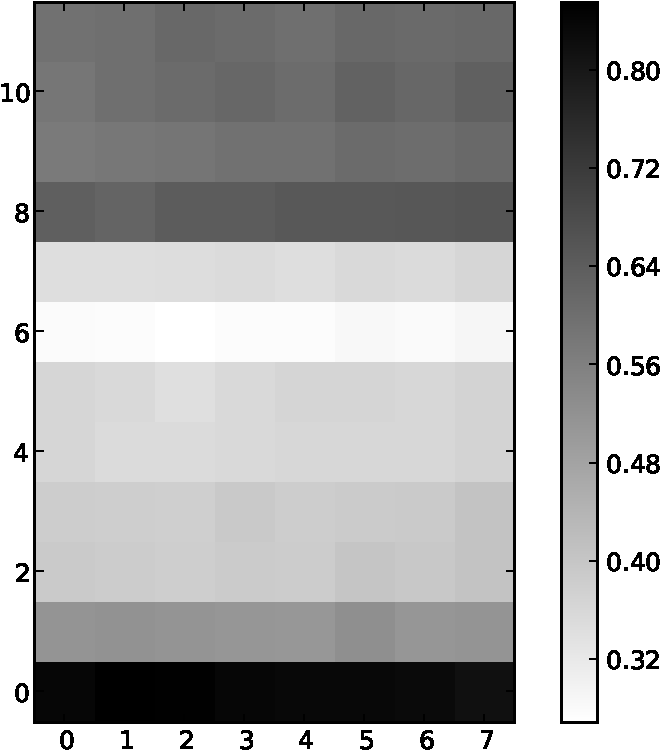
\includegraphics[width=0.32\columnwidth]{metallica_pattern}}
  \hspace{5mm}                
  \subfloat[][\small{Tori Amos / Suzanne Vega}]{\label{fig:amosvega2}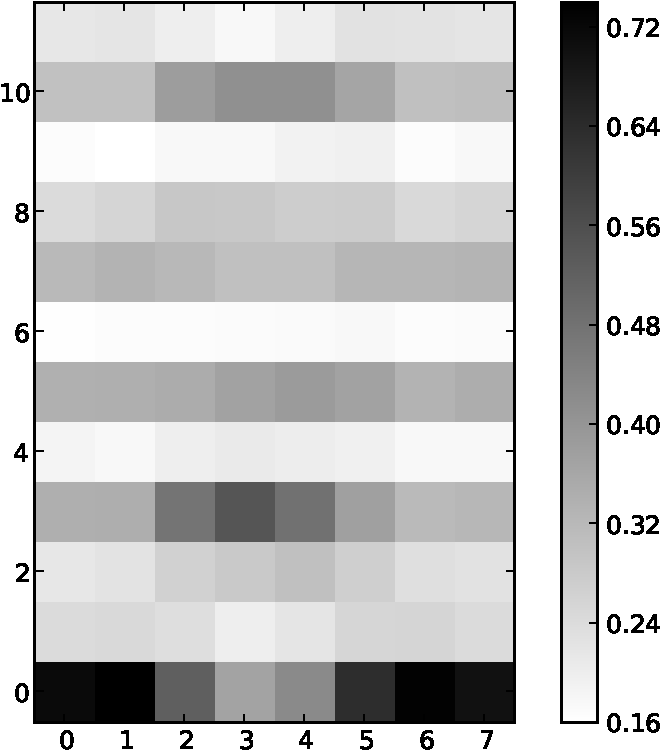
\includegraphics[width=0.32\columnwidth]{toriamos_suzannevega_pattern}}
  \vspace{2mm}
  \caption{\small{Typical patterns for different artists.}}
  \label{fig:typicalpat}
\end{figure}



\section{Conclusion and Future Work}
We have presented a practical method to perform large-scale clustering of
tonal patterns, and assessed the basic properties of the method through
experiments on a large collection of music. We have explored several ways
to inspect and interpret the data 
%(such as LLE) 
and suggested the merit of the representation
through further experiments.
We have discussed the possibility to move to even larger scales
and we provide our source code for other interested researchers.
\footnote{Code not yet released to preserve submission's anonymity}

Future work may include more sophisticated clustering that moves 
beyond simple Euclidean-distance-based quantization, perhaps 
by separately modeling the spread within each cluster (i.e., a Gaussian 
mixture or other generative model). 
%That being said, these methods
%could be use to develop better distance measures between patterns.
%The use of the euclidean distance is arbitrary. 
Summarizing patches
with Gaussians, and then comparing the distance between those Gaussians,
could reduce the influence of the noise in the distance measure.

Moving on to larger scales, we would like to pursue a scheme of incrementally 
splitting and merging codewords in response to a continuous, online stream 
of features, to create an increasingly-detailed, dynamic model.  We could
also cluster codebooks themselves, in a fashion similar to hierarchical
Gaussian mixtures \cite{Vasconcelos2001}.
%  (similar idea used for indexing \cite{Muja2009})


%\small
\section{Acknowledgements}
Thanks to Graham Grindlay for numerous discussions and helpful comments.
T. Bertin-Mahieux is supported by a NSERC scholarship.
This material is based upon work supported by the IMLS (grant LG-06-08-0073-08).


%\begin{thebibliography}{citations}
%\bibitem{Someone:04} 
%X. Someone and Y. Someone:
%{\it Title of the Book},
%Editorial Acme, Utrecht, 2004.
%\end{thebibliography}

\small
\bibliography{tbm_bib}





\end{document}
